\documentclass[../differential_geometry.tex]{subfiles}
\begin{document}
\section{Aula 11 -- 19 de Maio, 2026}
\subsection{Motivações}
\begin{itemize}
	\item Plano Hiperbólico;
	\item Ângulo entre Curvas em Superfícies;
	\item Áreas de Regiões de Superfícies.
\end{itemize}
\subsection{Plano Hiperbólico}

\begin{example}[O Plano Hiperbólico]
	Seja \(\underline{x}:U\subseteq \mathbb{R}^{2}\rightarrow S\) (não sabemos onde S mora) com \(U = \{(u, v)\in \mathbb{R}^{2}:\; v > 0\}\).
	Suponha que temos os seguintes coeficientes da primeira forma fundamental:
	\[
		E = \frac{1}{v^{2}},\; F = 0,\; \& \; G = \frac{1}{v^{2}},
	\]
	e considere a curva \(\alpha (t) = \underline{x}(0, t),\; v_{0}\leq t \leq v\), ou seja, que o traço da curva é a imagem por \(\underline{x}\) do segmento vertical \(u=0\) entre \(v_{0}\) e v.
	Então, o comprimento da curva \(\alpha \) em S é dado por
	\begin{align*}
		\ell (\alpha ) = \int_{v_{0}}^{v}\Vert \alpha '(t) \Vert \mathrm{d}t & = \int_{v0}^{v}[(u')^{2}E + 2u'v'F + (v')^{2}G]^{\frac{1}{2}} \mathrm{d}t \\
		                                                                     & = \int_{v_{0}}^{v}\sqrt[]{\frac{1}{t^{2}}} \mathrm{d}t                    \\
		                                                                     & = \int_{v_{0}}^{v}\frac{1}{t} \mathrm{d}t                                 \\
		                                                                     & = \ln^{}{\biggl(\frac{v}{v_{0}}\biggr)},
	\end{align*}
	e, em particular, conforme \(v_{0}\) se aproxima de 0, o limite do comprimento da curva tende ao infinito!

	Seja, agora, a curva \(\beta (t) = \underline{x}(t, v_{0})\), com \(-\pi \leq t \leq \pi \); temos, então,
	\[
		\ell (\beta ) = \int_{-\pi }^{\pi }[(u')^{2}E]^{\frac{1}{2}} \mathrm{d}t = \int_{-\pi }^{\pi }\frac{1}{v_{0}} \mathrm{d}t = \frac{2\pi }{v_{0}},
	\]
	de modo que
	\[
		\lim_{v_{0}\to 0}\ell (\beta ) = +\infty \quad\&\quad \lim_{v_{0}\to +\infty}\ell (\beta ) = 0.
	\]
	Fizemos as contas em S sem sequer saber onde ela fica!! Isso é mágico.
\end{example}
\begin{def*}
	O semiplano \(\{(u, v)\in \mathbb{R}^{2}:\; v > 0\} \) com a métrica \(\mathrm{d}s^{2} = \frac{1}{v^{2}}(\mathrm{d}u + \mathrm{d}v^{2})\) é chamado \textbf{plano hiperbólico,} denotado por \(\mathbb{H}.\; \square\)
\end{def*}

Surge a pergunta: será que existe \(\underline{x}:\mathbb{H}\rightarrow \mathbb{R}^{3}\) tal que a primeira forma fundamental de \(\underline{x}(\mathbb{H})\) é
\[
	\mathrm{d}s^{2} = \frac{1}{v^{2}}(\mathrm{d}u^{2} + \mathrm{d}v^{2})?
\]
Isso foi uma pergunta delicada, cuja resposta é não! (Hilbert, 1901); porém, uma região de \(\mathbb{H}\) pode ser realizada em \(\mathbb{R}^{3}\) -- consideramos
\[
	V = \{(u, v)\in \mathbb{R}^{2}:\; -\pi  < u < \pi ,\; v > 1\}
\]
e S como a superfície de revolução obtida ao girar a curva
\[
	\alpha (v) = \biggl(\frac{1}{v}, \mathrm{arcosh}^{}{(v)} - \frac{\sqrt[]{v^{2}-1}}{v}\biggr), \quad v >1,
\]
em torno do eixo z.
\begin{figure}[H]
	\begin{center}
		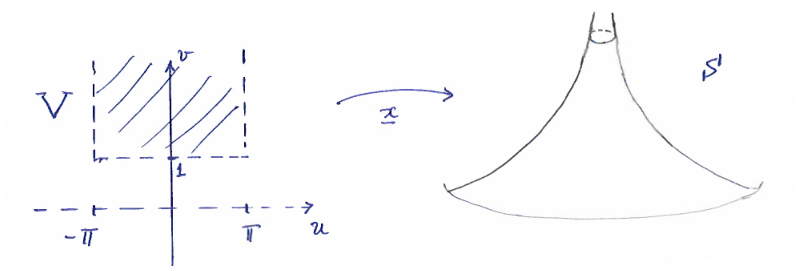
\includegraphics[height=\textheight, width=\textwidth, keepaspectratio]{./Images/hyperbolic_plane_11.png}
	\end{center}
\end{figure}
Na verdade, esse tema deu origem a um grande teorema da geometria, o
\hypertarget{nash_theorem}{
	\begin{theorem*}[Nash]
		Toda variedade Riemanniana pode ser mergulhada isometricamente em \(\mathbb{R}^{n}\) para algum n.
	\end{theorem*}
}
\subsection{Ângulo entre Curvas}
Adiante, seja S uma superfície e \(\underline{x}:U\subseteq \mathbb{R}^{2}\rightarrow S \subseteq \mathbb{R}^{n}\) uma parametrização local.
\begin{def*}
	Sejam \(\alpha_1,\; \alpha_2\) duas curvas em S com \(\alpha_1(t_1)=\alpha_2(t_2) = p\). O \textbf{ângulo entre \(\mathbf{\alpha_1}\) e \(\mathbf{\alpha_2}\)} em p é definido por
	\[
		\theta = \text{ângulo}(\alpha_1, \alpha_2) = \text{ângulo}(\alpha_1'(t_1), \alpha_2'(t_2)),
	\]
	e portanto como
	\[
		\boxed{\cos^{}{(\theta )} = \frac{\langle \alpha_1'(t_1), \alpha_2'(t_2)\rangle_{p}}{\Vert\alpha_1'(t_1) \Vert_{p} \Vert \alpha_{2}'(t_2) \Vert_p}} \; \square
	\]
\end{def*}
\begin{def*}
	\textbf{Curvas coordenadas} são as curvas parametrizadas por
	\begin{align*}
		 & t \mapsto \underline{x}(t, v_{0}), \quad (t, v_{0})\in U             \\
		 & t \mapsto \underline{x}(u_{0}, t), \quad (t, v_{0})\in U. \; \square
	\end{align*}
\end{def*}
Sejam \(\alpha_1(t) = \underline{x}(t, v_{0})\) e \(\alpha_2(s) = \underline{x}(u_{0}, s)\), com
\[
	\alpha_1(U_{0}) = \alpha_2(v_{0}) = \underline{x}(u_{0}, v_{0}).
\]
Em \(p = \underline{x}(u_{0}, v_{0})\), temos, para o \(\theta = \text{ângulo}(\alpha_1, \alpha_2)\), a seguinte relação:
\[
	\cos^{}{\theta } = \frac{\langle \alpha_1'(u_{0}), \alpha_2'(v_{0})\rangle_{p}}{\Vert \alpha_1'(u_{0}) \Vert_{p}\Vert \alpha_2'(v_{0}) \Vert_{p}} = \frac{\langle \underline{x}_{u}(u_{0}, v_{0}), \underline{x}_{v}(u_{0}, v_{0}) \rangle}{\Vert \underline{x}_{u}(u_{0}, v_{0}) \Vert \Vert \alpha_{2}'(v_{0}) \Vert},
\]
ou seja,
\[
	\cos^{}{(\theta )} = \frac{F}{\sqrt[]{EG}}.
\]
Em particular, as curvas coordenadas são ortogonais no ponto \(\underline{x}(u_{0}, v_{0})\) se, e somente se, \(F(u_{0},v_{0}) = 0\)

\subsection{Área de Regiões em uma Superfície}
Seja \(\underline{x}:U\subseteq \mathbb{R}^{2}\rightarrow S \subseteq \mathbb{R}^{n} \) uma parametrização local de S e seja \(\overline{R} = \underline{x}(R)\) uma região de \(\underline{x}(U)\subseteq S\).
Façamos R passar por uma subdivisão em retângulos com lados sendo segmentos de retas coordenadas em \(R\subseteq U\), ou seja,
\begin{figure}[H]
	\begin{center}
		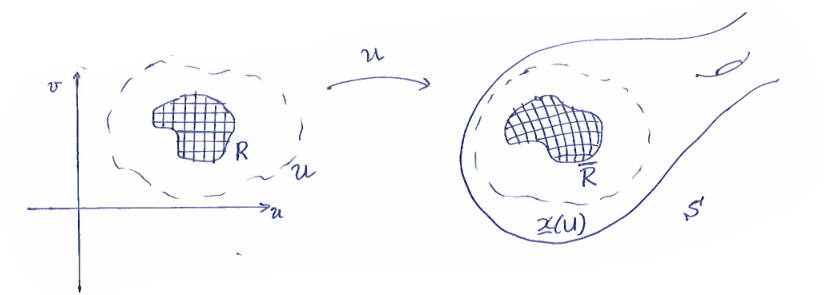
\includegraphics[height=\textheight, width=\textwidth, keepaspectratio]{./Images/region_area_11.png}
	\end{center}
\end{figure}

As imagens da subdivisão fornecem uma subdivisão de \(\overline{R}\) por curvas coordenadas! De fato, considere as curvas
\[
	\underline{x}(u_{0} + t\delta u, v_{0}) \quad\&\quad \underline{x}(u_{0}, v_{0}+t\delta v),\quad 0\leq t\leq 1,
\]
cujos vetores tangentes em \(t=0\) são
\begin{align*}
	 & \frac{\mathrm{d}}{\mathrm{d}t}(\underline{x}(u_{0}+t\delta u, v_{0}))\biggl|_{\mathrlap{t=0}}^{}\biggr. = \delta u\underline{x}_{u}(u_{0}, v_{0})  \\
	 & \frac{\mathrm{d}}{\mathrm{d}t}(\underline{x}(u_{0}, v_{0}+t\delta v))\biggl|_{\mathrlap{t=0}}^{}\biggr. = \delta v\underline{x}_{u}(u_{0}, v_{0}).
\end{align*}
Para \(\delta u\) e \(\delta v\) pequenos, o elemento de área pode ser aproximado pela área do paralelogramo de lados \(\delta u \underline{x}_{u}(u_{0}, v_{0})\) e \(\delta v \underline{x}_{v}(u_{0}, v_{0})\), que é
\[
	\delta A = \delta u \delta v \Vert \underline{x}_{u} \Vert \Vert \underline{x}_{v} \Vert\sin^{}{(\theta )} = \delta u \delta v\; \sqrt[]{EG}\sin^{}{(\theta )}.
\]
\begin{figure}[H]
	\begin{center}
		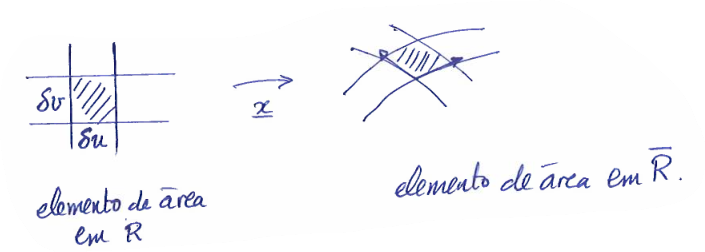
\includegraphics[height=\textheight, width=\textwidth, keepaspectratio]{./Images/subdivisions_11.png}
	\end{center}
\end{figure}
Daí, como \(\sin^{2}{\theta } = 1 - \cos^{2}{\theta },\) obtemos:
\begin{align*}
	\sin^{2}{\theta } = 1 - \frac{F^{2}}{EG} & = \frac{EG - F^{2}}{EG}                                  \\
	\Rightarrow                              & \boxed{\delta A = \sqrt[]{EG - F^{2}}\delta u \delta v}.
\end{align*}

\begin{def*}
	A \textbf{área da região \(\mathbf{\overline{R}}\)}, onde \(\overline{R} = \underline{x}(R)\), é definida por
	\[
		A(R) = \iint_{R}\sqrt[]{EG-F^{2}}\mathrm{d}u\mathrm{d}v. \; \square
	\]
\end{def*}
\begin{tcolorbox}[
		skin=enhanced,
		title=Observação,
		fonttitle=\bfseries,
		colframe=black,
		colbacktitle=cyan!75!white,
		colback=cyan!15,
		colbacklower=black,
		coltitle=black,
		drop fuzzy shadow,
		%drop large lifted shadow
	]
	Note que a definição depende somente da métrica!
\end{tcolorbox}
\begin{example}[Plano]
	No caso do plano dado por \(z=0\), ele pode ser parametrizado por
	\[
		\underline{x}(u, v) = (u, v, 0),
	\]
	tal que:
	\[
		E = 1, \; F= 0, \& G = 1.
	\]
	Consequentemente, a área do plano é dada pela integral dupla
	\[
		A(\overline{R}) = \iint_{R}\mathrm{d}u\mathrm{d}v.
	\]
\end{example}
\begin{example}[Esfera]
	Para uma esfera de raio r, a parametrização é
	\[
		\underline{x}(\theta , \varphi ) = (r\cos^{}{\theta }\cos^{}{\varphi }, r \cos^{}{\theta } \sin^{}{\varphi }, r \sin^{}{\theta }),
	\]
	onde
	\[
		(\theta , \varphi )\in U = \biggl\{(\theta , \varphi )\in \mathbb{R}^{2}:\; -\frac{\pi }{2} < \theta <\frac{\pi }{2},\; -\pi <\varphi <\pi \biggr\}.
	\]
	Observe que \(\underline{x}(U)\) é, na verdade, a esfera sem um meridiano e uma paralela. Neste exemplo, temos:
	\begin{align*}
		 & \underline{x}_{\theta } = (-r\sin^{}{\theta }\cos^{}{\varphi }, -r \sin^{}{\theta }\sin^{}{\varphi }, r \cos^{}{\theta }) \\
		 & \underline{x}_{\varphi } = (-r\cos^{}{\theta }\sin^{}{\varphi }, r\cos^{}{\theta }\cos^{}{\varphi }, 0),
	\end{align*}
	e, consequentemente, \(E = r^{2}, \; F = 0,\; G = r^{2}\cos^{2}{(\theta )}\); daí, o elemento de área da esfera é
	\[
		A(S^{2}(r)) = \iint_{U}\sqrt[]{EG-F^{2}}\mathrm{d}u\mathrm{d}v = \int_{-\frac{\pi }{2}}^{\frac{\pi }{2}} \int_{-\pi }^{\pi }r^{2}\cos^{}{(\theta )} \mathrm{d}\varphi  \mathrm{d}\theta  = 4\pi r^{2}.
	\]
\end{example}
\begin{example}[Plano Projetivo]
	De forma rápida, o elemento de área do plano projetivo é
	\[
		A(\overline{R}) = \int_{0}^{1}\int_{v_{0}}^{v_1}\frac{1}{v^{2}} \mathrm{d}u \mathrm{d}v = \biggl(-\frac{1}{v}\biggr)\biggl|_{v_{0}}^{v_1}\biggr. = \frac{1}{v_{0}}-\frac{1}{v_1}.
	\]
\end{example}
\end{document}

